\documentclass[border=6pt]{standalone}
\usepackage{tikz}
\usetikzlibrary{arrows.meta,calc,positioning}
\begin{document}
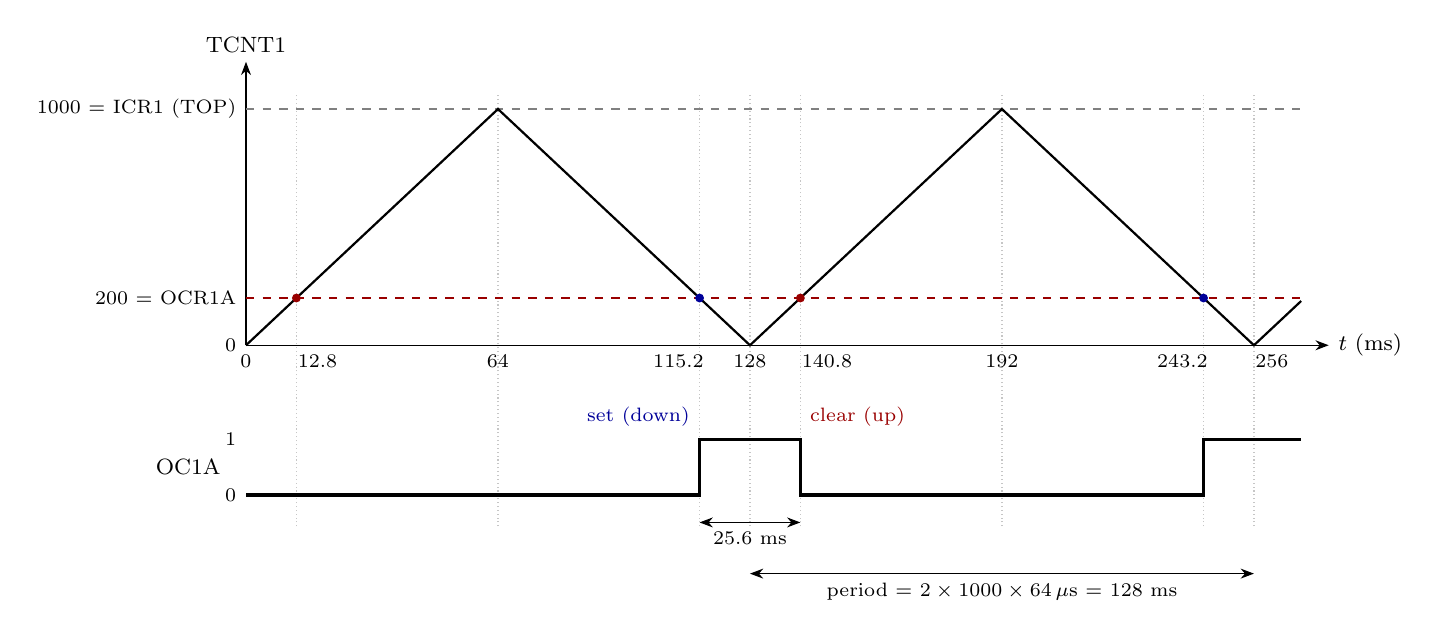
\begin{tikzpicture}[>=Stealth,font=\small,x=0.05cm,y=1cm]
% 1 unit = 1 ms; tick = 64 us; TOP = 1000 at 64 ms, BOTTOM at 128 ms; OCR1A = 200
% up-count matches: 12.8, 140.8 ms; down-count matches: 115.2, 243.2 ms
\def\H{3.0}\def\C{0.6}
\foreach \t in {12.8,64,115.2,128,140.8,192,243.2,256} \draw[gray!45,densely dotted] (\t,-2.3) -- (\t,\H+0.2);
\draw[->] (0,0) -- (0,\H+0.6) node[above,font=\footnotesize]{TCNT1};
\draw[->] (0,0) -- (275,0) node[right,font=\footnotesize]{$t$ (ms)};
\node[anchor=east,font=\scriptsize] at (0,\H) {1000 = ICR1 (TOP)};
\node[anchor=east,font=\scriptsize] at (0,\C) {200 = OCR1A};
\node[anchor=east,font=\scriptsize] at (0,0) {0};
\draw[gray,dashed] (0,\H) -- (268,\H);
\draw[red!60!black,dashed] (0,\C) -- (268,\C);
\draw[thick] (0,0) -- (64,\H) -- (128,0) -- (192,\H) -- (256,0) -- (268,{\H*12/64});
\foreach \t in {12.8,140.8} \fill[red!60!black] (\t,\C) circle (1.6pt);
\foreach \t in {115.2,243.2} \fill[blue!60!black] (\t,\C) circle (1.6pt);
\node[below,font=\scriptsize] at (0,0) {0};
\node[below right=0pt and -3pt,font=\scriptsize] at (12.8,0) {12.8};
\node[below,font=\scriptsize] at (64,0) {64};
\node[below left=0pt and -5pt,font=\scriptsize] at (115.2,0) {115.2};
\node[below,font=\scriptsize] at (128,0) {128};
\node[below right=0pt and -3pt,font=\scriptsize] at (140.8,0) {140.8};
\node[below,font=\scriptsize] at (192,0) {192};
\node[below left=0pt and -5pt,font=\scriptsize] at (243.2,0) {243.2};
\node[below right=0pt and -3pt,font=\scriptsize] at (256,0) {256};
\begin{scope}[yshift=-1.9cm]
\node[anchor=east,font=\footnotesize] at (-4,0.35) {OC1A};
\node[anchor=east,font=\scriptsize] at (0,0.7) {1};
\node[anchor=east,font=\scriptsize] at (0,0) {0};
\draw[very thick] (0,0) -- (115.2,0) -- (115.2,0.7) -- (140.8,0.7) -- (140.8,0) -- (243.2,0) -- (243.2,0.7) -- (268,0.7);
\node[font=\scriptsize,blue!60!black,anchor=south east] at (115.2,0.75) {set (down)};
\node[font=\scriptsize,red!60!black,anchor=south west] at (140.8,0.75) {clear (up)};
\draw[<->] (115.2,-0.35) -- (140.8,-0.35) node[midway,below,font=\scriptsize]{25.6 ms};
\draw[<->] (128,-1.0) -- (256,-1.0) node[midway,below,font=\scriptsize]{period = $2\times1000\times64\,\mu$s = 128 ms};
\end{scope}
\end{tikzpicture}
\end{document}
